\documentclass[10pt, b5paper, twoside]{extbook}
\usepackage[twoside,bindingoffset=10mm,verbose,marginratio={4:3,5:3},%
textwidth=143.3mm,height=218.6mm, nofoot, showframe]{geometry}

\usepackage[hyperfootnotes=false]{hyperref}
\usepackage{pdfpages}
\usepackage{fontspec}
\usepackage{fancyhdr}
\usepackage[compact, bottomtitles]{titlesec}
\usepackage{alphalph}
\usepackage[para, perpage]{footmisc}
\usepackage{footnpag}
\usepackage{graphicx}
\usepackage{svg}
\usepackage{ragged2e}
\usepackage{titletoc}
\usepackage{ifthen}
\usepackage[toc]{multitoc}
\usepackage{etoolbox}
\usepackage{alphalph}
\usepackage{paracol}
\usepackage{comment}
\usepackage{titlesec}
\usepackage{xcolor}
\usepackage[x-1a]{pdfx}
%\usepackage{bidi}
\usepackage{multicol}

\extrafloats{100}
\maxdeadcycles=200
\renewcommand{\thefootnote}{\alphalph{\value{footnote}}}
\renewcommand*{\multicolumntoc}{2}
\patchcmd{\makefootnoteparagraph}
   {\columnwidth}{\textwidth}
   {\typeout{Success}}{\typeout{patch failed}}

\setmainfont{BibleRoman}
            [UprightFont = *,
             BoldFont = *Bold,
             ItalicFont = *Italic,
             Ligatures=TeX]

\makeatletter             
\newlength\fake@f
\newlength\fake@c
\def\fakesc#1{%
  \begingroup%
  \xdef\fake@name{\csname\curr@fontshape/\f@size\endcsname}%
  \fontsize{\fontdimen8\fake@name}{\baselineskip}\selectfont%
  \uppercase{#1}%
  \endgroup%
}
\makeatother
\newcommand\fauxsc[1]{\fauxschelper#1 \relax\relax}
\def\fauxschelper#1 #2\relax{%
  \fauxschelphelp#1\relax\relax%
  \if\relax#2\relax\else\ \fauxschelper#2\relax\fi%
}
\def\Hscale{.83}\def\Vscale{.72}\def\Cscale{1.00}
\def\fauxschelphelp#1#2\relax{%
  \ifnum`#1=\lccode`#1\relax\scalebox{\Hscale}[\Vscale]{\char\uccode`#1}\else%
    \scalebox{\Cscale}[1]{#1}\fi%
  \ifx\relax#2\relax\else\fauxschelphelp#2\relax\fi}

\renewcommand{\textsc}[1]{{\fauxsc{#1}}}
\renewcommand{\emph}[1]{{\textit{#1}}}

\pagestyle{fancy}
\renewcommand{\sectionmark}[1]{\markright{\thesection~- ~#1}}
\renewcommand{\chaptermark}[1]{\markboth{\chaptername~\thechapter~-~ #1}{}}
\pagestyle{empty}

\titleformat{\chapter}[display]
  {\normalfont\bfseries}{}{0pt}{\Huge}

\fancyhf{}

\fancypagestyle{bible}{%
    \fancyhead{} %Clean headers
    \fancyhead[L]{\leftmark \ \thesection}
    \fancyhead[R]{\thepage}
    \fancyhead[RO]{\leftmark \ \thesection}
    \fancyhead[LO]{\thepage}
}

\fancypagestyle{plain}{%
  \fancyhead{}
  \fancyhead[R, RO]{\thepage}
}

\renewcommand{\chaptermark}[1]{\markboth{\thechapter. {\slshape{##1}}}{}}
\renewcommand{\headrulewidth}{0pt}
% \renewcommand*{\thefootnote}{\alph{footnote}}
\titleformat{\chapter}[hang]{\normalfont\bfseries}{}{0pt}{\Huge}
\titleformat{\section}[wrap]{\bfseries\huge}{}{0ex}{}[]
\titleformat{\subsection}[hang]{\bfseries}{}{0ex}{}[]
\newcommand{\bibleverse}[1]{{\bfseries{#1}}}
\newcommand{\wordsOfJesus}[1]{{#1}}
\renewcommand{\thesection}{\arabic{section}}
\renewcommand{\chaptermark}[1]{\markboth{\MakeUppercase{#1}}{}}
\setcounter{secnumdepth}{1}
\setcounter{tocdepth}{0}
\global\let\endtitlepage\relax
\makeatletter

\titlecontents{chapter}% <section-type>
[0pt]% <left>
{\bfseries\small}% <above-code>
{\small\thecontentslabel \quad}%<numbered-entry-format>
{}% <numberless-entry-format>
{\small\mdseries\titlerule*[0.75em]{.}\bfseries\contentspage}

\defaultfontfeatures{Scale=MatchLowercase} %so that different fonts have same xheight
\newfontfamily\hebrewfont[Script=Hebrew]{Frank Ruehl CLM}
\newfontfamily\greekfont[Script=Greek]{Cardo}
\newcommand{\hebrew}[1]{{\hebrewfont{#1}}}
\newcommand{\greek}[1]{{\greekfont{#1}}}

\newcommand{\biblebeginparacol}{\begin{paracol}{2}}
\newcommand{\bibleendparacol}{\end{paracol}}

\begin{document}

\includepdf{FrontCover.pdf}

\null\vfill
\begin{center}
\begin{minipage}[c]{\textwidth}
  \begin{center}
  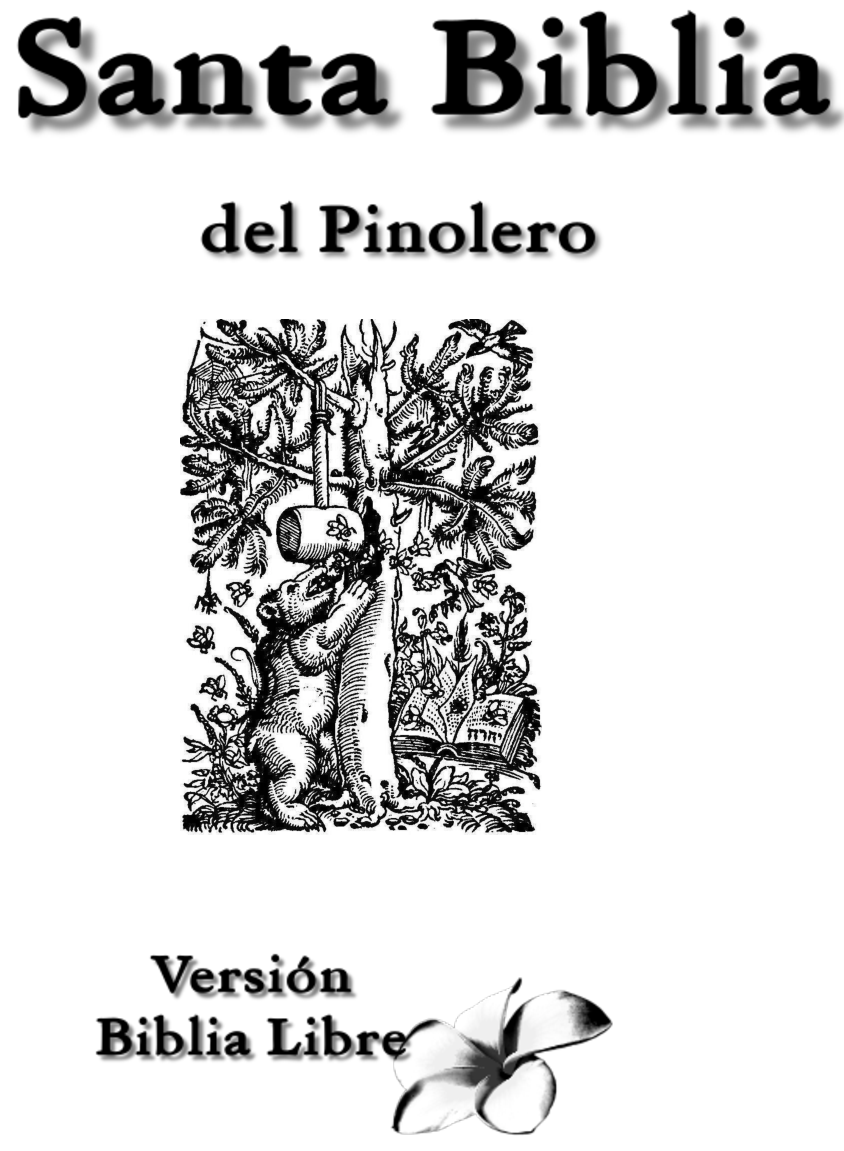
\includegraphics{Titulo.pdf}
  \end{center}
\end{minipage}
\end{center}
\newpage

\null\vfill
\noindent
Reina-Valera del Pueblo, Version 2021\\
dominio publico y fuente abierta,\\
creado por el ministerio Biblia del Pueblo\\
basado sobre el texto de la Reina-Valera 1909\\

\noindent
1ra edición 2021\\

\noindent
ISBN \dots\\

\noindent
\emph{Distribucion en Nicaragua}\\
Estrellas de Esperanza\\
Reparto santa Rosa de donde fue la hielera del yanki\\
media cuadra al sur o vien de donde es la carpinteria\\
media al sur casa color celeste\\
43000 Granada\\
Nicaragua\\
ventas@estrellasdeesperanza.org\\
www.estrellasdeesperanza.org\\

\noindent
Derechos dominio publico, el texto de la Biblia es fuente abierta\\
con una licencia de MIT.\\
El código fuente de markdown y LaTeX se encuentra en github en\\
http://www.github.com/simonegli8/FreeBible\\
Reina-Valera del Pueblo es una marca comercial registrado por Biblia del Pueblo\\
Los derechos publicar modificationes del codigo fuente abierto original con la marca Reina-Valera del Pueblo
son reservado. Si vosostro publican modificaciones del texto biblico del codigo fuente abierta original, es prohibido
utilizar la marca Reina-Valera del Pueblo, necessita cambiar el nombre de la traduccion, pero si no cambian el texto biblico es permitio. El prefacio y gloassario no son parte
del texto biblico, y se puebe modificarlo voluntariamente.\\

\noindent
Imprenta: Imprenta Jigatsa, Managua, Nicaragua\\
\newpage

\titleformat{\section}[hang]{\bfseries\huge}{}{0ex}{}[]
\input{tex/00-prefacio.tex}
\titleformat{\section}[wrap]{\bfseries\huge}{}{0ex}{}[]

\tableofcontents
\newpage

\null\vfill
\begin{center}
\begin{minipage}[c]{\textwidth}
  \begin{center}
  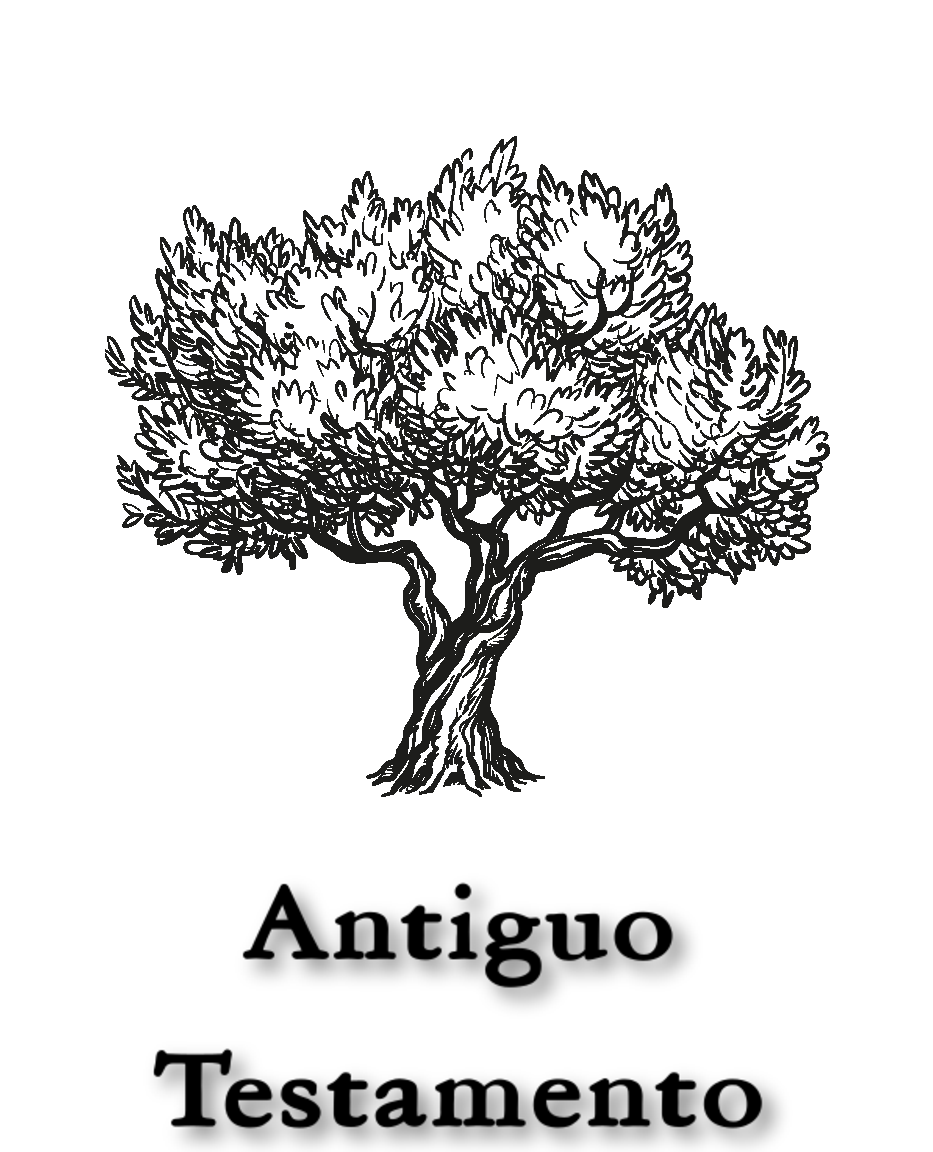
\includegraphics{AntiguoTestamentoTitulo.pdf}
  \end{center}
\end{minipage}
\end{center}
\null\vfill
\newpage

\pagestyle{bible}

\renewcommand{\cleardoublepage}{}
\renewcommand{\clearpage}{}

\chapter{Génesis}
\begin{multicols}{2}
  \input{tex/01-Génesis.tex}
\end{multicols}

\chapter{Salmos}
\begin{multicols}{2}
  \input{tex/19-Salmos.tex}
\end{multicols}

\chapter{Proverbios}
\begin{multicols}{2}
  \input{tex/20-Proverbios.tex}
\end{multicols}
\newpage

\pagestyle{empty}

\null\vfill
\begin{center}
\begin{minipage}[c]{\textwidth}
  \begin{center}
  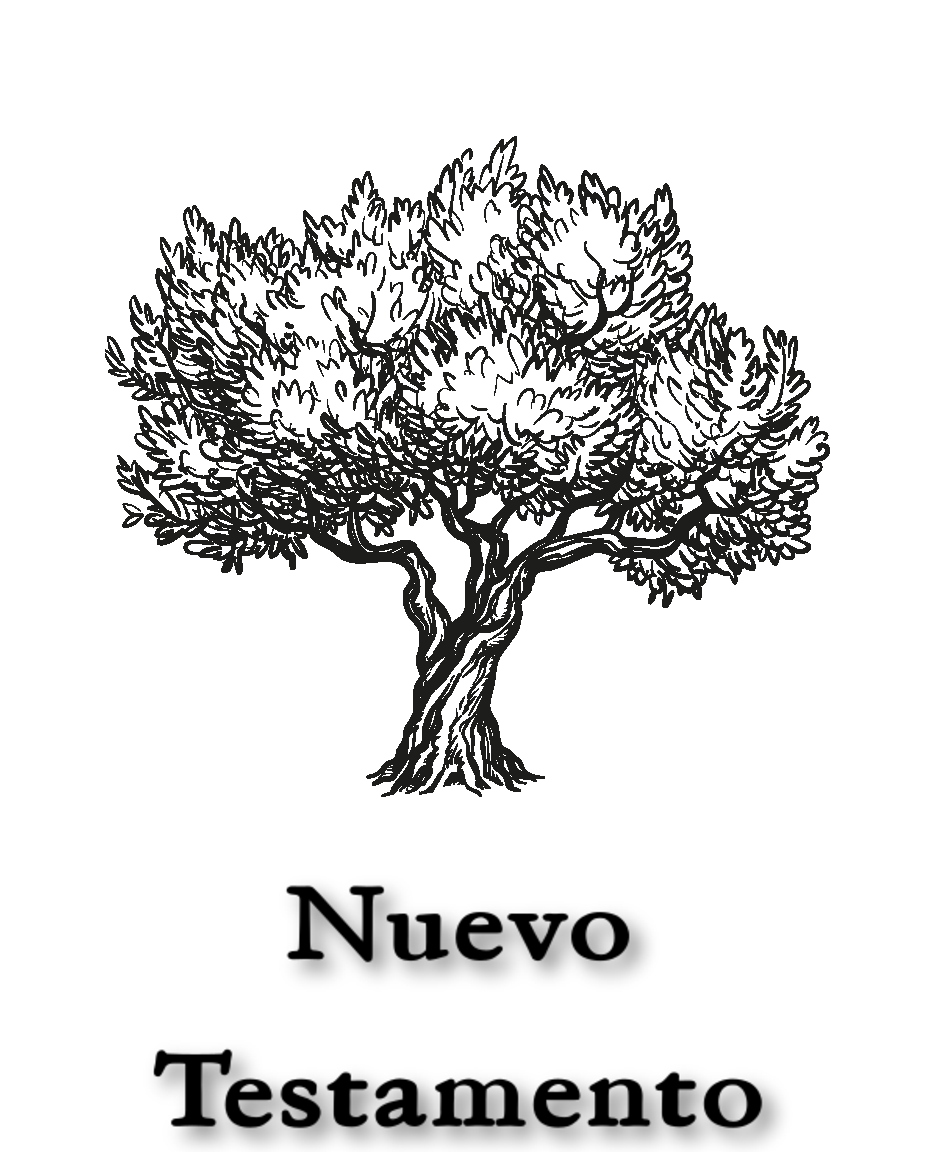
\includegraphics{NuevoTestamentoTitulo.pdf}
  \end{center}
\end{minipage}
\end{center}
\null\vfill

\end{document}